% Options for packages loaded elsewhere
\PassOptionsToPackage{unicode}{hyperref}
\PassOptionsToPackage{hyphens}{url}
%
\documentclass[
  11pt,
  ignorenonframetext,
  svgnames, handout, t]{beamer}
\usepackage{pgfpages}
\setbeamertemplate{caption}[numbered]
\setbeamertemplate{caption label separator}{: }
\setbeamercolor{caption name}{fg=normal text.fg}
\beamertemplatenavigationsymbolsempty
% Prevent slide breaks in the middle of a paragraph
\widowpenalties 1 10000
\raggedbottom
\setbeamertemplate{part page}{
  \centering
  \begin{beamercolorbox}[sep=16pt,center]{part title}
    \usebeamerfont{part title}\insertpart\par
  \end{beamercolorbox}
}
\setbeamertemplate{section page}{
  \centering
  \begin{beamercolorbox}[sep=12pt,center]{part title}
    \usebeamerfont{section title}\insertsection\par
  \end{beamercolorbox}
}
\setbeamertemplate{subsection page}{
  \centering
  \begin{beamercolorbox}[sep=8pt,center]{part title}
    \usebeamerfont{subsection title}\insertsubsection\par
  \end{beamercolorbox}
}
\AtBeginPart{
  \frame{\partpage}
}
\AtBeginSection{
  \ifbibliography
  \else
    \frame{\sectionpage}
  \fi
}
\AtBeginSubsection{
  \frame{\subsectionpage}
}
\usepackage{amsmath,amssymb}
\usepackage{lmodern}
\usepackage{iftex}
\ifPDFTeX
  \usepackage[T1]{fontenc}
  \usepackage[utf8]{inputenc}
  \usepackage{textcomp} % provide euro and other symbols
\else % if luatex or xetex
  \usepackage{unicode-math}
  \defaultfontfeatures{Scale=MatchLowercase}
  \defaultfontfeatures[\rmfamily]{Ligatures=TeX,Scale=1}
\fi
\usefonttheme{professionalfonts}
% Use upquote if available, for straight quotes in verbatim environments
\IfFileExists{upquote.sty}{\usepackage{upquote}}{}
\IfFileExists{microtype.sty}{% use microtype if available
  \usepackage[]{microtype}
  \UseMicrotypeSet[protrusion]{basicmath} % disable protrusion for tt fonts
}{}
\makeatletter
\@ifundefined{KOMAClassName}{% if non-KOMA class
  \IfFileExists{parskip.sty}{%
    \usepackage{parskip}
  }{% else
    \setlength{\parindent}{0pt}
    \setlength{\parskip}{6pt plus 2pt minus 1pt}}
}{% if KOMA class
  \KOMAoptions{parskip=half}}
\makeatother
\usepackage{xcolor}
\IfFileExists{xurl.sty}{\usepackage{xurl}}{} % add URL line breaks if available
\IfFileExists{bookmark.sty}{\usepackage{bookmark}}{\usepackage{hyperref}}
\hypersetup{
  pdftitle={Distribution of Hourly Earnings by Age},
  pdfauthor={Patrick Toche },
  hidelinks,
  pdfcreator={LaTeX via pandoc}}
\urlstyle{same} % disable monospaced font for URLs
\newif\ifbibliography
\usepackage{color}
\usepackage{fancyvrb}
\newcommand{\VerbBar}{|}
\newcommand{\VERB}{\Verb[commandchars=\\\{\}]}
\DefineVerbatimEnvironment{Highlighting}{Verbatim}{commandchars=\\\{\}}
% Add ',fontsize=\small' for more characters per line
\usepackage{framed}
\definecolor{shadecolor}{RGB}{248,248,248}
\newenvironment{Shaded}{\begin{snugshade}}{\end{snugshade}}
\newcommand{\AlertTok}[1]{\textcolor[rgb]{0.94,0.16,0.16}{#1}}
\newcommand{\AnnotationTok}[1]{\textcolor[rgb]{0.56,0.35,0.01}{\textbf{\textit{#1}}}}
\newcommand{\AttributeTok}[1]{\textcolor[rgb]{0.77,0.63,0.00}{#1}}
\newcommand{\BaseNTok}[1]{\textcolor[rgb]{0.00,0.00,0.81}{#1}}
\newcommand{\BuiltInTok}[1]{#1}
\newcommand{\CharTok}[1]{\textcolor[rgb]{0.31,0.60,0.02}{#1}}
\newcommand{\CommentTok}[1]{\textcolor[rgb]{0.56,0.35,0.01}{\textit{#1}}}
\newcommand{\CommentVarTok}[1]{\textcolor[rgb]{0.56,0.35,0.01}{\textbf{\textit{#1}}}}
\newcommand{\ConstantTok}[1]{\textcolor[rgb]{0.00,0.00,0.00}{#1}}
\newcommand{\ControlFlowTok}[1]{\textcolor[rgb]{0.13,0.29,0.53}{\textbf{#1}}}
\newcommand{\DataTypeTok}[1]{\textcolor[rgb]{0.13,0.29,0.53}{#1}}
\newcommand{\DecValTok}[1]{\textcolor[rgb]{0.00,0.00,0.81}{#1}}
\newcommand{\DocumentationTok}[1]{\textcolor[rgb]{0.56,0.35,0.01}{\textbf{\textit{#1}}}}
\newcommand{\ErrorTok}[1]{\textcolor[rgb]{0.64,0.00,0.00}{\textbf{#1}}}
\newcommand{\ExtensionTok}[1]{#1}
\newcommand{\FloatTok}[1]{\textcolor[rgb]{0.00,0.00,0.81}{#1}}
\newcommand{\FunctionTok}[1]{\textcolor[rgb]{0.00,0.00,0.00}{#1}}
\newcommand{\ImportTok}[1]{#1}
\newcommand{\InformationTok}[1]{\textcolor[rgb]{0.56,0.35,0.01}{\textbf{\textit{#1}}}}
\newcommand{\KeywordTok}[1]{\textcolor[rgb]{0.13,0.29,0.53}{\textbf{#1}}}
\newcommand{\NormalTok}[1]{#1}
\newcommand{\OperatorTok}[1]{\textcolor[rgb]{0.81,0.36,0.00}{\textbf{#1}}}
\newcommand{\OtherTok}[1]{\textcolor[rgb]{0.56,0.35,0.01}{#1}}
\newcommand{\PreprocessorTok}[1]{\textcolor[rgb]{0.56,0.35,0.01}{\textit{#1}}}
\newcommand{\RegionMarkerTok}[1]{#1}
\newcommand{\SpecialCharTok}[1]{\textcolor[rgb]{0.00,0.00,0.00}{#1}}
\newcommand{\SpecialStringTok}[1]{\textcolor[rgb]{0.31,0.60,0.02}{#1}}
\newcommand{\StringTok}[1]{\textcolor[rgb]{0.31,0.60,0.02}{#1}}
\newcommand{\VariableTok}[1]{\textcolor[rgb]{0.00,0.00,0.00}{#1}}
\newcommand{\VerbatimStringTok}[1]{\textcolor[rgb]{0.31,0.60,0.02}{#1}}
\newcommand{\WarningTok}[1]{\textcolor[rgb]{0.56,0.35,0.01}{\textbf{\textit{#1}}}}
\usepackage{graphicx}
\makeatletter
\def\maxwidth{\ifdim\Gin@nat@width>\linewidth\linewidth\else\Gin@nat@width\fi}
\def\maxheight{\ifdim\Gin@nat@height>\textheight\textheight\else\Gin@nat@height\fi}
\makeatother
% Scale images if necessary, so that they will not overflow the page
% margins by default, and it is still possible to overwrite the defaults
% using explicit options in \includegraphics[width, height, ...]{}
\setkeys{Gin}{width=\maxwidth,height=\maxheight,keepaspectratio}
% Set default figure placement to htbp
\makeatletter
\def\fps@figure{htbp}
\makeatother
\setlength{\emergencystretch}{3em} % prevent overfull lines
\providecommand{\tightlist}{%
  \setlength{\itemsep}{0pt}\setlength{\parskip}{0pt}}
\setcounter{secnumdepth}{-\maxdimen} % remove section numbering
\geometry{paperwidth=160mm,paperheight=106mm}
\usepackage{lmodern}% bug: converts \pounds to dollar sign
\usepackage[english]{babel}
\usepackage[T1]{fontenc}% font encoding, load before inputenc
\usepackage{fontspec}% font encoding
\frenchspacing
\defaultfontfeatures{
   Mapping=tex-text,
   Scale=MatchLowercase,
}
%   \setsansfont{Montserrat}
\setsansfont{Lato}
\setmonofont{Droid Sans Mono}
\newfontfamily\fontbold{Lato Bold}
\newfontfamily\fontitalic{Lato Italic}
\newfontfamily\fontbolditalic{Lato Bold Italic}
\newfontfamily\quotefont{Minotaur}

\usepackage{amsmath}
\usepackage{graphicx}
\usepackage{caption}
\usepackage{hyperref}

\colorlet{themetext}{black}
\colorlet{themefill}{RoyalBlue!50}
\colorlet{themecolor}{NavyBlue}
\usetheme{default}
\setbeamertemplate{navigation symbols}{}
\setbeamercovered{transparent}
\setbeamertemplate{title page}[empty]
\usecolortheme{seahorse}
\setbeamercovered{transparent=4}
\setbeamercolor{palette primary}{use=structure,fg=black,bg=themefill}
\setbeamercolor{title}{fg=black}
\setbeamercolor{frametitle}{fg=black}
\setbeamercolor{itemize item}{fg=themecolor}
\setbeamercolor{enumerate item}{fg=themecolor}
\setbeamercolor{itemize subitem}{fg=themecolor}
\setbeamercolor{enumerate subitem}{fg=themecolor}
%\setbeamertemplate{itemize item}[triangle]% default, triangle, circle, square, ball
\setbeamertemplate{itemize item}{\raisebox{-0.7ex}{\scalebox{1}[2.5]{\bfseries\textendash}}} 
\setbeamertemplate{itemize subitem}{\raisebox{-0.7ex}{\scalebox{1}[2.5]{\bfseries\textendash}}} 
\setbeamertemplate{enumerate subitem}{\alph{enumii}.}
\ifLuaTeX
  \usepackage{selnolig}  % disable illegal ligatures
\fi

\title{Distribution of Hourly Earnings by Age}
\subtitle{Econ 440 - Introduction to Econometrics}
\author{Patrick Toche}
\date{19 February 2022}

\begin{document}
\frame{\titlepage}

\begin{frame}{Objectives}
\protect\hypertarget{objectives}{}
\begin{enumerate}
\tightlist
\item
  Compute the marginal distribution of Age.
\item
  Compute the mean of AHE for each value of Age.
\item
  Plot the mean of AHE versus Age.
\item
  Compute the variance of AHE.
\item
  Compute the covariance between AHE and Age.
\item
  Compute the correlation between AHE and Age.
\end{enumerate}
\end{frame}

\begin{frame}[fragile]{Why use R}
\protect\hypertarget{why-use-r}{}
The convenience of programming over spreadsheets is that you can run
multiple calculations in a few lines of code and, as a result, you can
reproduce your results quickly, and share your calculations easily. With
a spreadsheet, you typically need to use the menus and mouse multiple
times and replication is not so straightforward.

\texttt{R} is open-source, free software that is popular for statistical
calculations. An alternative is \texttt{Python}, also open source and
free.

Each have their strengths and weaknesses.

One of the best things about \texttt{R} is the \texttt{RStudio}
interface and the \texttt{tidyverse} family of packages, particularly
the plotting library \texttt{ggplot2}.

One of the best things about \texttt{Python} is its huge and increasing
following, particularly in machine learning.

For data-heavy project, consider \texttt{Julia}, another wonderful
open-source project.
\end{frame}

\begin{frame}[fragile]{Set Up Working Directory}
\protect\hypertarget{set-up-working-directory}{}
The working directory is where R/Rstudio will search for data files and
where it will save objects you create.

If you're on Windows, set your working directly with:

\footnotesize

\begin{Shaded}
\begin{Highlighting}[]
    \FunctionTok{setwd}\NormalTok{(}\StringTok{"c:/R/workspace"}\NormalTok{)}
\end{Highlighting}
\end{Shaded}

\normalsize

If you're on MacOS, use

\footnotesize

\begin{Shaded}
\begin{Highlighting}[]
    \FunctionTok{setwd}\NormalTok{(}\StringTok{"\textasciitilde{}/R/workspace"}\NormalTok{)}
\end{Highlighting}
\end{Shaded}

\normalsize where \texttt{\textasciitilde{}} is a short-hand for the
path to the user directory.

The condition below checks your operating system and sets a working
directory accordingly.

\footnotesize

\begin{Shaded}
\begin{Highlighting}[]
\CommentTok{\# useful if you switch from Windows to Mac/Linux: }
\ControlFlowTok{if}\NormalTok{(.Platform}\SpecialCharTok{$}\NormalTok{OS.type }\SpecialCharTok{==} \StringTok{"windows"}\NormalTok{)\{}
    \FunctionTok{setwd}\NormalTok{(}\StringTok{"c:/R/workspace"}\NormalTok{)}
\NormalTok{\} }\ControlFlowTok{else}\NormalTok{ \{}
    \FunctionTok{setwd}\NormalTok{(}\StringTok{"\textasciitilde{}/R/workspace"}\NormalTok{)}
\NormalTok{\}}
\end{Highlighting}
\end{Shaded}

\normalsize Check that you're in the right place with

\footnotesize

\begin{Shaded}
\begin{Highlighting}[]
    \FunctionTok{getwd}\NormalTok{()}
\end{Highlighting}
\end{Shaded}

\normalsize
\end{frame}

\begin{frame}[fragile]{Set Options}
\protect\hypertarget{set-options}{}
To reduce the number of significant digits that are printed in the
console, you may set the \texttt{digits} option:

\footnotesize

\begin{Shaded}
\begin{Highlighting}[]
\FunctionTok{library}\NormalTok{(}\StringTok{"readxl"}\NormalTok{)}
\FunctionTok{options}\NormalTok{(}\AttributeTok{digits=}\DecValTok{4}\NormalTok{)}
\end{Highlighting}
\end{Shaded}

\normalsize

If you are working with time series data, you may find the
\texttt{digits.secs} option useful,

\footnotesize

\begin{Shaded}
\begin{Highlighting}[]
\FunctionTok{library}\NormalTok{(}\StringTok{"readxl"}\NormalTok{)}
\FunctionTok{options}\NormalTok{(}\AttributeTok{digits.secs=}\DecValTok{2}\NormalTok{)}
\end{Highlighting}
\end{Shaded}

\normalsize

Another useful option to limit or increase the output printed to the
console is \texttt{max.print},

\footnotesize

\begin{Shaded}
\begin{Highlighting}[]
\FunctionTok{library}\NormalTok{(}\StringTok{"readxl"}\NormalTok{)}
\FunctionTok{options}\NormalTok{(}\AttributeTok{max.print=}\DecValTok{5}\NormalTok{)}
\end{Highlighting}
\end{Shaded}

\normalsize

Note that in R, the period is a character like any other. In Python it
is not, so the naming convention would most likely be one of
\texttt{maxprint} or \texttt{MaxPrint}. In Python, the use of
underscores, as in \texttt{max\_print}, is usually preferred for
functions, with the ``camel'\,' notation preferred for variable names,
but not everyone follows these guidelines. In R, the use of dots in
variable names and function arguments is popular.
\end{frame}

\begin{frame}[fragile]{Install Packages}
\protect\hypertarget{install-packages}{}
In R, packages are also called libraries.

In order to use a package, you first need to install it:

\footnotesize

\begin{Shaded}
\begin{Highlighting}[]
\FunctionTok{add.packages}\NormalTok{(}\StringTok{"readxl"}\NormalTok{)}
\end{Highlighting}
\end{Shaded}

\normalsize

And before you use it, you must load it with the \texttt{library()}
function,

\footnotesize

\begin{Shaded}
\begin{Highlighting}[]
\FunctionTok{library}\NormalTok{(}\StringTok{"readxl"}\NormalTok{)}
\end{Highlighting}
\end{Shaded}

\normalsize

Once in a while, remember to update your existing packages, with

\footnotesize

\begin{Shaded}
\begin{Highlighting}[]
\FunctionTok{update.packages}\NormalTok{()}
\end{Highlighting}
\end{Shaded}

\normalsize The above will attempt to update all your packages. This is
generally a good idea, though it could occasionally break your code if
the package has experienced an overhaul.

If you need to install a package from source -- an older version of a
popular package or an experimental package not available via the usual
distribution channels:

\footnotesize

\begin{Shaded}
\begin{Highlighting}[]
\NormalTok{url }\OtherTok{\textless{}{-}} \StringTok{"http://cran.r{-}project.org/src/contrib/Archive/ggplot2/ggplot2\_0.9.1.tar.gz"}
\FunctionTok{install.packages}\NormalTok{(url, }\AttributeTok{repos=}\ConstantTok{NULL}\NormalTok{, }\AttributeTok{type=}\StringTok{"source"}\NormalTok{)}
\end{Highlighting}
\end{Shaded}

\normalsize Not recommended unless an update has broken your code and
you are under a tight deadline!
\end{frame}

\begin{frame}[fragile]{Read the Data}
\protect\hypertarget{read-the-data}{}
The data is in \texttt{xlsx} format: One way to read it is with the
\texttt{readxl} library. This creates a \texttt{tibble} (part of
\texttt{tidyverse}) rather than the standard \texttt{dataframe} (base
R).

\footnotesize

\begin{Shaded}
\begin{Highlighting}[]
\FunctionTok{library}\NormalTok{(}\StringTok{"readxl"}\NormalTok{)  }\CommentTok{\# remember to load the package beforehand}
\NormalTok{data }\OtherTok{\textless{}{-}} \FunctionTok{read\_xlsx}\NormalTok{(}\StringTok{"Age\_HourlyEarnings.xlsx"}\NormalTok{)}
\end{Highlighting}
\end{Shaded}

\normalsize

\begin{itemize}
\item
  We are using the \texttt{read\_xlsx} function from the package
  \texttt{readxl}.
\item
  We are assigning the result of applying the \texttt{read\_xlsx}
  function to the variable name \texttt{data}
\end{itemize}

In R, assignments are bi-directional, so we could also do:

\footnotesize

\begin{Shaded}
\begin{Highlighting}[]
\FunctionTok{library}\NormalTok{(}\StringTok{"readxl"}\NormalTok{)}
\FunctionTok{read\_xlsx}\NormalTok{(}\StringTok{"Age\_HourlyEarnings.xlsx"}\NormalTok{) }\OtherTok{{-}\textgreater{}}\NormalTok{ data}
\end{Highlighting}
\end{Shaded}

\normalsize

An assignment could also be done with the equal sign,

\footnotesize

\begin{Shaded}
\begin{Highlighting}[]
\FunctionTok{library}\NormalTok{(}\StringTok{"readxl"}\NormalTok{)}
\NormalTok{data }\OtherTok{=} \FunctionTok{read\_xlsx}\NormalTok{(}\StringTok{"Age\_HourlyEarnings.xlsx"}\NormalTok{)}
\end{Highlighting}
\end{Shaded}

\normalsize

Was the data loaded correctly?

\footnotesize

\begin{Shaded}
\begin{Highlighting}[]
\FunctionTok{View}\NormalTok{(data)  }\CommentTok{\# Note the capital V in View!}
\end{Highlighting}
\end{Shaded}

\normalsize
\end{frame}

\begin{frame}[fragile]{Read the Data}
\protect\hypertarget{read-the-data-1}{}
More control: takes some trial and error to get it right!

\footnotesize

\begin{Shaded}
\begin{Highlighting}[]
\FunctionTok{library}\NormalTok{(}\StringTok{"readxl"}\NormalTok{)}
\NormalTok{df1 }\OtherTok{\textless{}{-}} \FunctionTok{read\_xlsx}\NormalTok{(}\StringTok{"Age\_HourlyEarnings.xlsx"}\NormalTok{,}
                  \AttributeTok{col\_names=}\ConstantTok{TRUE}\NormalTok{,}
                  \AttributeTok{skip=}\DecValTok{1}\NormalTok{,}
                  \AttributeTok{trim\_ws=}\ConstantTok{TRUE}\NormalTok{)}
\end{Highlighting}
\end{Shaded}

\normalsize

\begin{itemize}
\item
  Set \texttt{col\_names=TRUE} to use the ages as column names
\item
  Skip the first line with \texttt{skip=1}
\item
  Trim white space with \texttt{trim\_ws}, because white spaces can mess
  things up in ways that are difficult to debug.
\item
  See more options with \texttt{?read\_xlsx}
\end{itemize}
\end{frame}

\begin{frame}[fragile]{Quick View of the Data}
\protect\hypertarget{quick-view-of-the-data}{}
Our data may be accessed with the name \texttt{df1}. We will clean it
and, as we do, overwrite it at each iteration. However, when you are
debugging your own data, it is recommended that you use a different
name, say \texttt{df1.tmp}, and check that everything is as expected
before renaming it \texttt{df1} and overwriting the data.

The dataframe \texttt{df1} is in \textbf{wide format}. We will convert
it to \textbf{long format} and name the new dataframe \texttt{df2}. We
will use \texttt{df1} or \texttt{df2} whenever the format is most
convenient for our purpose.

Quickly view a slice of the data with \texttt{head(df1)}:

\footnotesize

\begin{Shaded}
\begin{Highlighting}[]
\FunctionTok{head}\NormalTok{(df1)}
\CommentTok{\#\textgreater{} \# A tibble: 6 x 13}
\CommentTok{\#\textgreater{}     AHE    \textasciigrave{}25\textasciigrave{}    \textasciigrave{}26\textasciigrave{}    \textasciigrave{}27\textasciigrave{}    \textasciigrave{}28\textasciigrave{}    \textasciigrave{}29\textasciigrave{}    \textasciigrave{}30\textasciigrave{}     \textasciigrave{}31\textasciigrave{}    \textasciigrave{}32\textasciigrave{}    \textasciigrave{}33\textasciigrave{}}
\CommentTok{\#\textgreater{}   \textless{}dbl\textgreater{}   \textless{}dbl\textgreater{}   \textless{}dbl\textgreater{}   \textless{}dbl\textgreater{}   \textless{}dbl\textgreater{}   \textless{}dbl\textgreater{}   \textless{}dbl\textgreater{}    \textless{}dbl\textgreater{}   \textless{}dbl\textgreater{}   \textless{}dbl\textgreater{}}
\CommentTok{\#\textgreater{} 1     5 0.00298 0.00218 0.00204 0.00211 0.00145 0.00153 0.00131  0.00102 0.00145}
\CommentTok{\#\textgreater{} 2     6 0.00116 0.00167 0.00109 0.00109 0.00131 0.00109 0.000509 0.00174 0.00102}
\CommentTok{\#\textgreater{} 3     7 0.00247 0.00262 0.00254 0.00167 0.00283 0.00240 0.00174  0.00189 0.00204}
\CommentTok{\#\textgreater{} 4     8 0.00240 0.00225 0.00167 0.00240 0.00138 0.00276 0.00218  0.00174 0.00211}
\CommentTok{\#\textgreater{} 5     9 0.00356 0.00327 0.00283 0.00291 0.00320 0.00240 0.00262  0.00196 0.00305}
\CommentTok{\#\textgreater{} 6    10 0.00516 0.00523 0.00400 0.00523 0.00443 0.00451 0.00458  0.00414 0.00480}
\CommentTok{\#\textgreater{} \# ... with 3 more variables: \textasciigrave{}34\textasciigrave{} \textless{}dbl\textgreater{}, ...12 \textless{}lgl\textgreater{}, ...13 \textless{}lgl\textgreater{}}
\end{Highlighting}
\end{Shaded}

\normalsize
\end{frame}

\begin{frame}[fragile]{Quick View of the Data}
\protect\hypertarget{quick-view-of-the-data-1}{}
View less or more of the data by setting the second argument of
\texttt{head()}

\footnotesize

\begin{Shaded}
\begin{Highlighting}[]
\FunctionTok{head}\NormalTok{(df1, }\DecValTok{2}\NormalTok{)}
\CommentTok{\#\textgreater{} \# A tibble: 2 x 13}
\CommentTok{\#\textgreater{}     AHE    \textasciigrave{}25\textasciigrave{}    \textasciigrave{}26\textasciigrave{}    \textasciigrave{}27\textasciigrave{}    \textasciigrave{}28\textasciigrave{}    \textasciigrave{}29\textasciigrave{}    \textasciigrave{}30\textasciigrave{}     \textasciigrave{}31\textasciigrave{}    \textasciigrave{}32\textasciigrave{}    \textasciigrave{}33\textasciigrave{}}
\CommentTok{\#\textgreater{}   \textless{}dbl\textgreater{}   \textless{}dbl\textgreater{}   \textless{}dbl\textgreater{}   \textless{}dbl\textgreater{}   \textless{}dbl\textgreater{}   \textless{}dbl\textgreater{}   \textless{}dbl\textgreater{}    \textless{}dbl\textgreater{}   \textless{}dbl\textgreater{}   \textless{}dbl\textgreater{}}
\CommentTok{\#\textgreater{} 1     5 0.00298 0.00218 0.00204 0.00211 0.00145 0.00153 0.00131  0.00102 0.00145}
\CommentTok{\#\textgreater{} 2     6 0.00116 0.00167 0.00109 0.00109 0.00131 0.00109 0.000509 0.00174 0.00102}
\CommentTok{\#\textgreater{} \# ... with 3 more variables: \textasciigrave{}34\textasciigrave{} \textless{}dbl\textgreater{}, ...12 \textless{}lgl\textgreater{}, ...13 \textless{}lgl\textgreater{}}
\end{Highlighting}
\end{Shaded}

\normalsize

or look at the tail \texttt{tail(df1)}:

\footnotesize

\begin{Shaded}
\begin{Highlighting}[]
\FunctionTok{tail}\NormalTok{(df1, }\DecValTok{4}\NormalTok{)}
\CommentTok{\#\textgreater{} \# A tibble: 4 x 13}
\CommentTok{\#\textgreater{}     AHE      \textasciigrave{}25\textasciigrave{}     \textasciigrave{}26\textasciigrave{}     \textasciigrave{}27\textasciigrave{}     \textasciigrave{}28\textasciigrave{}     \textasciigrave{}29\textasciigrave{}     \textasciigrave{}30\textasciigrave{}     \textasciigrave{}31\textasciigrave{}     \textasciigrave{}32\textasciigrave{}}
\CommentTok{\#\textgreater{}   \textless{}dbl\textgreater{}     \textless{}dbl\textgreater{}    \textless{}dbl\textgreater{}    \textless{}dbl\textgreater{}    \textless{}dbl\textgreater{}    \textless{}dbl\textgreater{}    \textless{}dbl\textgreater{}    \textless{}dbl\textgreater{}    \textless{}dbl\textgreater{}}
\CommentTok{\#\textgreater{} 1    65   7.27e{-}5  2.91e{-}4  1.45e{-}4  2.91e{-}4  3.63e{-}4  4.36e{-}4  5.09e{-}4  0.00102}
\CommentTok{\#\textgreater{} 2    70   5.09e{-}4  9.45e{-}4  4.36e{-}4  1.16e{-}3  1.16e{-}3  1.31e{-}3  1.31e{-}3  0.00313}
\CommentTok{\#\textgreater{} 3    NA  NA       NA       NA       NA       NA       NA       NA       NA      }
\CommentTok{\#\textgreater{} 4    NA  NA       NA       NA       NA       NA       NA       NA       NA      }
\CommentTok{\#\textgreater{} \# ... with 4 more variables: \textasciigrave{}33\textasciigrave{} \textless{}dbl\textgreater{}, \textasciigrave{}34\textasciigrave{} \textless{}dbl\textgreater{}, ...12 \textless{}lgl\textgreater{}, ...13 \textless{}lgl\textgreater{}}
\end{Highlighting}
\end{Shaded}

\normalsize
\end{frame}

\begin{frame}[fragile]{Quick View of the Data}
\protect\hypertarget{quick-view-of-the-data-2}{}
A few things are apparent from viewing the data in the console, that may
not have been immediately obvious from the display of \texttt{View()}

The column names are strings:

\footnotesize

\begin{Shaded}
\begin{Highlighting}[]
\FunctionTok{colnames}\NormalTok{(df1)}
\CommentTok{\#\textgreater{}  [1] "AHE"   "25"    "26"    "27"    "28"    "29"    "30"    "31"    "32"   }
\CommentTok{\#\textgreater{} [10] "33"    "34"    "...12" "...13"}
\end{Highlighting}
\end{Shaded}

\normalsize

In R, a string is called a character, it is usually displayed with
quote-marks, as in ``25''.

There are missing values -- those are the \texttt{NA} values.

The variables described as \texttt{\textless{}dbl\textgreater{}} are
double-precision floating-point number -- as opposed to, say, integers.
\end{frame}

\begin{frame}[fragile]{Quick View of the Data}
\protect\hypertarget{quick-view-of-the-data-3}{}
We see missing values in the last rows of the dataframe, but the output
of \texttt{head()} and \texttt{tail()} is truncated before the last
columns, where there are more missing values. These missing values are
not apparent from viewing the spreadsheet in Excel, but they could be
seen with \texttt{View(df1)}.

Viewing a selected slice of the dataframe:

\footnotesize

\begin{Shaded}
\begin{Highlighting}[]
\NormalTok{df1[}\FunctionTok{ncol}\NormalTok{(df1)]  }\CommentTok{\# last column}
\CommentTok{\#\textgreater{} \# A tibble: 31 x 1}
\CommentTok{\#\textgreater{}    ...13}
\CommentTok{\#\textgreater{}    \textless{}lgl\textgreater{}}
\CommentTok{\#\textgreater{}  1 NA   }
\CommentTok{\#\textgreater{}  2 NA   }
\CommentTok{\#\textgreater{}  3 NA   }
\CommentTok{\#\textgreater{}  4 NA   }
\CommentTok{\#\textgreater{}  5 NA   }
\CommentTok{\#\textgreater{}  6 NA   }
\CommentTok{\#\textgreater{}  7 NA   }
\CommentTok{\#\textgreater{}  8 NA   }
\CommentTok{\#\textgreater{}  9 NA   }
\CommentTok{\#\textgreater{} 10 NA   }
\CommentTok{\#\textgreater{} \# ... with 21 more rows}
\end{Highlighting}
\end{Shaded}

\normalsize where \texttt{ncol()} counts the number of columns -- There
is also \texttt{nrow()}.
\end{frame}

\begin{frame}[fragile]{Quick View of the Data}
\protect\hypertarget{quick-view-of-the-data-4}{}
Viewing a selected slice of the dataframe:

\footnotesize

\begin{Shaded}
\begin{Highlighting}[]
\NormalTok{df1[,(}\FunctionTok{ncol}\NormalTok{(df1)}\SpecialCharTok{{-}}\DecValTok{4}\NormalTok{)}\SpecialCharTok{:}\FunctionTok{ncol}\NormalTok{(df1)]  }\CommentTok{\# last 5 columns}
\CommentTok{\#\textgreater{} \# A tibble: 31 x 5}
\CommentTok{\#\textgreater{}       \textasciigrave{}32\textasciigrave{}    \textasciigrave{}33\textasciigrave{}    \textasciigrave{}34\textasciigrave{} ...12 ...13}
\CommentTok{\#\textgreater{}      \textless{}dbl\textgreater{}   \textless{}dbl\textgreater{}   \textless{}dbl\textgreater{} \textless{}lgl\textgreater{} \textless{}lgl\textgreater{}}
\CommentTok{\#\textgreater{}  1 0.00102 0.00145 0.00102 NA    NA   }
\CommentTok{\#\textgreater{}  2 0.00174 0.00102 0.00124 NA    NA   }
\CommentTok{\#\textgreater{}  3 0.00189 0.00204 0.00182 NA    NA   }
\CommentTok{\#\textgreater{}  4 0.00174 0.00211 0.00225 NA    NA   }
\CommentTok{\#\textgreater{}  5 0.00196 0.00305 0.00204 NA    NA   }
\CommentTok{\#\textgreater{}  6 0.00414 0.00480 0.00363 NA    NA   }
\CommentTok{\#\textgreater{}  7 0.00349 0.00283 0.00334 NA    NA   }
\CommentTok{\#\textgreater{}  8 0.00669 0.00574 0.00661 NA    NA   }
\CommentTok{\#\textgreater{}  9 0.00371 0.00392 0.00392 NA    NA   }
\CommentTok{\#\textgreater{} 10 0.00574 0.00523 0.00661 NA    NA   }
\CommentTok{\#\textgreater{} \# ... with 21 more rows}
\end{Highlighting}
\end{Shaded}

\normalsize
\end{frame}

\begin{frame}[fragile]{Quick View of the Data}
\protect\hypertarget{quick-view-of-the-data-5}{}
Viewing a selected slice of the dataframe:

\footnotesize

\begin{Shaded}
\begin{Highlighting}[]
\NormalTok{df1[}\DecValTok{6}\SpecialCharTok{:}\DecValTok{7}\NormalTok{]  }\CommentTok{\# if you know exactly which columns to select}
\CommentTok{\#\textgreater{} \# A tibble: 31 x 2}
\CommentTok{\#\textgreater{}       \textasciigrave{}29\textasciigrave{}    \textasciigrave{}30\textasciigrave{}}
\CommentTok{\#\textgreater{}      \textless{}dbl\textgreater{}   \textless{}dbl\textgreater{}}
\CommentTok{\#\textgreater{}  1 0.00145 0.00153}
\CommentTok{\#\textgreater{}  2 0.00131 0.00109}
\CommentTok{\#\textgreater{}  3 0.00283 0.00240}
\CommentTok{\#\textgreater{}  4 0.00138 0.00276}
\CommentTok{\#\textgreater{}  5 0.00320 0.00240}
\CommentTok{\#\textgreater{}  6 0.00443 0.00451}
\CommentTok{\#\textgreater{}  7 0.00371 0.00269}
\CommentTok{\#\textgreater{}  8 0.00705 0.00727}
\CommentTok{\#\textgreater{}  9 0.00429 0.00443}
\CommentTok{\#\textgreater{} 10 0.00690 0.00661}
\CommentTok{\#\textgreater{} \# ... with 21 more rows}
\end{Highlighting}
\end{Shaded}

\normalsize
\end{frame}

\begin{frame}[fragile]{Quick View of the Data}
\protect\hypertarget{quick-view-of-the-data-6}{}
with tidyverse pipe \textbar{} displays in reverse order:

\footnotesize

\begin{Shaded}
\begin{Highlighting}[]
\FunctionTok{library}\NormalTok{(tidyverse)}
\NormalTok{df1 }\SpecialCharTok{\%\textgreater{}\%} \FunctionTok{select}\NormalTok{(}\FunctionTok{last\_col}\NormalTok{(}\AttributeTok{offset=}\DecValTok{0}\SpecialCharTok{:}\DecValTok{4}\NormalTok{), }\FunctionTok{everything}\NormalTok{()) }\SpecialCharTok{\%\textgreater{}\%} \FunctionTok{head}\NormalTok{(}\DecValTok{5}\NormalTok{)}
\CommentTok{\#\textgreater{} \# A tibble: 5 x 13}
\CommentTok{\#\textgreater{}   ...13 ...12    \textasciigrave{}34\textasciigrave{}    \textasciigrave{}33\textasciigrave{}    \textasciigrave{}32\textasciigrave{}   AHE    \textasciigrave{}25\textasciigrave{}    \textasciigrave{}26\textasciigrave{}    \textasciigrave{}27\textasciigrave{}    \textasciigrave{}28\textasciigrave{}}
\CommentTok{\#\textgreater{}   \textless{}lgl\textgreater{} \textless{}lgl\textgreater{}   \textless{}dbl\textgreater{}   \textless{}dbl\textgreater{}   \textless{}dbl\textgreater{} \textless{}dbl\textgreater{}   \textless{}dbl\textgreater{}   \textless{}dbl\textgreater{}   \textless{}dbl\textgreater{}   \textless{}dbl\textgreater{}}
\CommentTok{\#\textgreater{} 1 NA    NA    0.00102 0.00145 0.00102     5 0.00298 0.00218 0.00204 0.00211}
\CommentTok{\#\textgreater{} 2 NA    NA    0.00124 0.00102 0.00174     6 0.00116 0.00167 0.00109 0.00109}
\CommentTok{\#\textgreater{} 3 NA    NA    0.00182 0.00204 0.00189     7 0.00247 0.00262 0.00254 0.00167}
\CommentTok{\#\textgreater{} 4 NA    NA    0.00225 0.00211 0.00174     8 0.00240 0.00225 0.00167 0.00240}
\CommentTok{\#\textgreater{} 5 NA    NA    0.00204 0.00305 0.00196     9 0.00356 0.00327 0.00283 0.00291}
\CommentTok{\#\textgreater{} \# ... with 3 more variables: \textasciigrave{}29\textasciigrave{} \textless{}dbl\textgreater{}, \textasciigrave{}30\textasciigrave{} \textless{}dbl\textgreater{}, \textasciigrave{}31\textasciigrave{} \textless{}dbl\textgreater{}}
\end{Highlighting}
\end{Shaded}

\normalsize

The \texttt{\%\textgreater{}\%} symbol is a ``pipe'' to conveniently
transforme the original \texttt{tibble} in a series of stages,
convenient for debugging.

The \texttt{\%\textgreater{}\%} pipe is from the \texttt{tidyverse}
family, not from base R.
\end{frame}

\begin{frame}[fragile]{Quick View of the Data}
\protect\hypertarget{quick-view-of-the-data-7}{}
A more compact display of the last column:

\footnotesize

\begin{Shaded}
\begin{Highlighting}[]
\FunctionTok{library}\NormalTok{(tidyverse)}
\NormalTok{df1[}\FunctionTok{ncol}\NormalTok{(df1)] }\SpecialCharTok{\%\textgreater{}\%}\NormalTok{ data.frame }\SpecialCharTok{\%\textgreater{}\%} \FunctionTok{head}\NormalTok{(}\DecValTok{5}\NormalTok{)}
\CommentTok{\#\textgreater{}   ...13}
\CommentTok{\#\textgreater{} 1    NA}
\CommentTok{\#\textgreater{} 2    NA}
\CommentTok{\#\textgreater{} 3    NA}
\CommentTok{\#\textgreater{} 4    NA}
\CommentTok{\#\textgreater{} 5    NA}
\end{Highlighting}
\end{Shaded}

\normalsize Here we transform the \texttt{tibble} to a dataframe before
displaying the \texttt{head}. A dataframe has a more compact display.

The default \texttt{dataframe} does not support integers as names and
therefore prepends an \texttt{X}: ``25'' becomes ``X25''. In
\texttt{tidyverse}, the \texttt{tibble} is an extension of the
\texttt{dataframe} which supports numbers as column names. Let's see
that now.
\end{frame}

\begin{frame}[fragile]{Read the Data as CSV}
\protect\hypertarget{read-the-data-as-csv}{}
It is often convenient to work with \texttt{csv} files (\texttt{csv}
stands for comma-separated values), because \texttt{csv} files have a
simple structure and can be read with other statistical software.

Save the excel spreadsheet as a plain \texttt{csv} file and open it
with:

\footnotesize

\begin{Shaded}
\begin{Highlighting}[]
\NormalTok{df1.csv }\OtherTok{\textless{}{-}} \FunctionTok{read.csv}\NormalTok{(}\StringTok{"Age\_HourlyEarnings.csv"}\NormalTok{, }
                    \AttributeTok{skip=}\DecValTok{1}\NormalTok{, }
                    \AttributeTok{header=}\ConstantTok{TRUE}\NormalTok{, }
                    \AttributeTok{stringsAsFactors=}\ConstantTok{FALSE}\NormalTok{)}
\end{Highlighting}
\end{Shaded}

\normalsize

Most of the time, you want to make sure that strings are not converted
to factors. This is done with the argument
\texttt{stringsAsFactors=FALSE}, which is otherwise set to \texttt{TRUE}
by default.

By contrast, \texttt{readxl} does not convert strings as factors by
default.

Let's see the differences between \texttt{df1} and this \texttt{df}. We
can check the structure of an object with \texttt{str()}.
\end{frame}

\begin{frame}[fragile]{Compare dataframe and tibble}
\protect\hypertarget{compare-dataframe-and-tibble}{}
This is the structure of the data imported with \texttt{read\_xlsx()}:

\footnotesize

\begin{Shaded}
\begin{Highlighting}[]
\FunctionTok{str}\NormalTok{(df1)}
\CommentTok{\#\textgreater{} tibble [31 x 13] (S3: tbl\_df/tbl/data.frame)}
\CommentTok{\#\textgreater{}  $ AHE  : num [1:31] 5 6 7 8 9 10 11 12 13 14 ...}
\CommentTok{\#\textgreater{}  $ 25   : num [1:31] 0.00298 0.00116 0.00247 0.0024 0.00356 ...}
\CommentTok{\#\textgreater{}  $ 26   : num [1:31] 0.00218 0.00167 0.00262 0.00225 0.00327 ...}
\CommentTok{\#\textgreater{}  $ 27   : num [1:31] 0.00204 0.00109 0.00254 0.00167 0.00283 ...}
\CommentTok{\#\textgreater{}  $ 28   : num [1:31] 0.00211 0.00109 0.00167 0.0024 0.00291 ...}
\CommentTok{\#\textgreater{}  $ 29   : num [1:31] 0.00145 0.00131 0.00283 0.00138 0.0032 ...}
\CommentTok{\#\textgreater{}  $ 30   : num [1:31] 0.00153 0.00109 0.0024 0.00276 0.0024 ...}
\CommentTok{\#\textgreater{}  $ 31   : num [1:31] 0.001308 0.000509 0.001744 0.00218 0.002616 ...}
\CommentTok{\#\textgreater{}  $ 32   : num [1:31] 0.00102 0.00174 0.00189 0.00174 0.00196 ...}
\CommentTok{\#\textgreater{}  $ 33   : num [1:31] 0.00145 0.00102 0.00204 0.00211 0.00305 ...}
\CommentTok{\#\textgreater{}  $ 34   : num [1:31] 0.00102 0.00124 0.00182 0.00225 0.00204 ...}
\CommentTok{\#\textgreater{}  $ ...12: logi [1:31] NA NA NA NA NA NA ...}
\CommentTok{\#\textgreater{}  $ ...13: logi [1:31] NA NA NA NA NA NA ...}
\end{Highlighting}
\end{Shaded}

\normalsize
\end{frame}

\begin{frame}[fragile]{Compare dataframe and tibble}
\protect\hypertarget{compare-dataframe-and-tibble-1}{}
This is the structure of the data imported with \texttt{read.csv()}:

\footnotesize

\begin{Shaded}
\begin{Highlighting}[]
\FunctionTok{str}\NormalTok{(df1.csv)}
\CommentTok{\#\textgreater{} \textquotesingle{}data.frame\textquotesingle{}:    31 obs. of  13 variables:}
\CommentTok{\#\textgreater{}  $ AHE: int  5 6 7 8 9 10 11 12 13 14 ...}
\CommentTok{\#\textgreater{}  $ X25: num  0.00298 0.00116 0.00247 0.0024 0.00356 ...}
\CommentTok{\#\textgreater{}  $ X26: num  0.00218 0.00167 0.00262 0.00225 0.00327 ...}
\CommentTok{\#\textgreater{}  $ X27: num  0.00204 0.00109 0.00254 0.00167 0.00283 ...}
\CommentTok{\#\textgreater{}  $ X28: num  0.00211 0.00109 0.00167 0.0024 0.00291 ...}
\CommentTok{\#\textgreater{}  $ X29: num  0.00145 0.00131 0.00283 0.00138 0.0032 ...}
\CommentTok{\#\textgreater{}  $ X30: num  0.00153 0.00109 0.0024 0.00276 0.0024 ...}
\CommentTok{\#\textgreater{}  $ X31: num  0.001308 0.000509 0.001744 0.00218 0.002616 ...}
\CommentTok{\#\textgreater{}  $ X32: num  0.00102 0.00174 0.00189 0.00174 0.00196 ...}
\CommentTok{\#\textgreater{}  $ X33: num  0.00145 0.00102 0.00204 0.00211 0.00305 ...}
\CommentTok{\#\textgreater{}  $ X34: num  0.00102 0.00124 0.00182 0.00225 0.00204 ...}
\CommentTok{\#\textgreater{}  $ X  : logi  NA NA NA NA NA NA ...}
\CommentTok{\#\textgreater{}  $ X.1: logi  NA NA NA NA NA NA ...}
\end{Highlighting}
\end{Shaded}

\normalsize
\end{frame}

\begin{frame}[fragile]{Compare dataframe and tibble}
\protect\hypertarget{compare-dataframe-and-tibble-2}{}
The \texttt{tibble} is a modern evolution of the \texttt{dataframe}
available in base \texttt{R}. It is part of the family of packages
developed by RStudio and Hadley Wickham that go under the name
\texttt{tidyverse}. The description states ``The tidyverse is an
opinionated collection of R packages designed for data science.''

These packages include, among others:

\begin{itemize}
\tightlist
\item
  \texttt{ggplot2} the most popular plotting library
\item
  \texttt{scales} a companion to \texttt{ggplot2} that assists in
  scaling axes and formatting labels
\item
  \texttt{dplyr}, \texttt{tidyr} provide various utilities to
  conveniently manipulate data.
\item
  \texttt{readxl} to read excel files and convert them to a
  \texttt{tibble}
\item
  \texttt{stringr} to manipulate strings
\item
  \texttt{forcats}, \texttt{readr}, \texttt{purr}, etc.
\end{itemize}

Go to \url{https://www.tidyverse.org/} and download the cheatsheets

Older, now deprecated packages that people still use include
\texttt{plyr}, \texttt{reshape2}.

\begin{itemize}
\tightlist
\item
  Be careful if you use both \texttt{plyr} and \texttt{dplyr} because
  they both use a \texttt{summarise} function, and unexpected results
  can occur. Instead of \texttt{summarise}, write
  \texttt{dplyr::summarise} or \texttt{plyr::summarise} to make sure you
  are using the desired function.
\end{itemize}
\end{frame}

\begin{frame}[fragile]{Clean the Data}
\protect\hypertarget{clean-the-data}{}
Check basic information:

\footnotesize

\begin{Shaded}
\begin{Highlighting}[]
\FunctionTok{nrow}\NormalTok{(df1)}
\FunctionTok{ncol}\NormalTok{(df1)}
\FunctionTok{colnames}\NormalTok{(df1)}
\FunctionTok{is.na}\NormalTok{(df1)}
\FunctionTok{complete.cases}\NormalTok{(df1)}
\end{Highlighting}
\end{Shaded}

\normalsize

Remove empty columns:

\footnotesize

\begin{Shaded}
\begin{Highlighting}[]
\NormalTok{df1 }\OtherTok{\textless{}{-}} \FunctionTok{Filter}\NormalTok{(}\ControlFlowTok{function}\NormalTok{(x)}\SpecialCharTok{!}\FunctionTok{all}\NormalTok{(}\FunctionTok{is.na}\NormalTok{(x)), df1)}
\end{Highlighting}
\end{Shaded}

\normalsize

Remove empty columns, including empty strings and 0 values:

\footnotesize

\begin{Shaded}
\begin{Highlighting}[]
\FunctionTok{Filter}\NormalTok{(}\ControlFlowTok{function}\NormalTok{(x)}\SpecialCharTok{!}\FunctionTok{all}\NormalTok{(}\FunctionTok{is.na}\NormalTok{(x) }\SpecialCharTok{||} \FunctionTok{is.null}\NormalTok{(x) }\SpecialCharTok{||}\NormalTok{ x }\SpecialCharTok{==} \StringTok{""} \SpecialCharTok{||}\NormalTok{ x }\SpecialCharTok{==} \DecValTok{0}\NormalTok{), df1)}
\end{Highlighting}
\end{Shaded}

\normalsize

See if any rows have missing values:

\footnotesize

\begin{Shaded}
\begin{Highlighting}[]
\FunctionTok{complete.cases}\NormalTok{(df1)}
\CommentTok{\#\textgreater{}  [1]  TRUE  TRUE  TRUE  TRUE  TRUE  TRUE  TRUE  TRUE  TRUE  TRUE  TRUE  TRUE}
\CommentTok{\#\textgreater{} [13]  TRUE  TRUE  TRUE  TRUE  TRUE  TRUE  TRUE  TRUE  TRUE  TRUE  TRUE  TRUE}
\CommentTok{\#\textgreater{} [25]  TRUE  TRUE  TRUE  TRUE  TRUE FALSE FALSE}
\end{Highlighting}
\end{Shaded}

\normalsize The last two rows have missing values!
\end{frame}

\begin{frame}[fragile]{Clean the Data}
\protect\hypertarget{clean-the-data-1}{}
Remove empty rows:

\footnotesize

\begin{Shaded}
\begin{Highlighting}[]
\NormalTok{df1 }\OtherTok{\textless{}{-}}\NormalTok{ df1[}\FunctionTok{complete.cases}\NormalTok{(df1), ] }
\end{Highlighting}
\end{Shaded}

\normalsize

Save cleaned data:

\footnotesize

\begin{Shaded}
\begin{Highlighting}[]
\FunctionTok{save}\NormalTok{(df1, }\AttributeTok{file =} \StringTok{"Age\_HourlyEarnings\_clean\_wide.RData"}\NormalTok{)}
\end{Highlighting}
\end{Shaded}

\normalsize

Or see below how to save to a \texttt{csv} or to an \texttt{xlsx} file.
\end{frame}

\begin{frame}[fragile]{Clean the Data \textbar{} with dplyr}
\protect\hypertarget{clean-the-data-with-dplyr}{}
The \texttt{dplyr} does certain things more intuitively than base
\texttt{R}. Let's clean the data again!

\footnotesize

\begin{Shaded}
\begin{Highlighting}[]
\NormalTok{df1 }\OtherTok{\textless{}{-}} \FunctionTok{read\_xlsx}\NormalTok{(}\StringTok{"Age\_HourlyEarnings.xlsx"}\NormalTok{, }\AttributeTok{col\_names=}\ConstantTok{TRUE}\NormalTok{, }\AttributeTok{skip=}\DecValTok{1}\NormalTok{, }\AttributeTok{trim\_ws=}\ConstantTok{TRUE}\NormalTok{)}
\end{Highlighting}
\end{Shaded}

\normalsize

Because there are missing values in both the rows and the columns, we
have to proceed with caution. It would be tempting to do this:

\footnotesize

\begin{Shaded}
\begin{Highlighting}[]
\NormalTok{df1 }\SpecialCharTok{\%\textgreater{}\%} \FunctionTok{filter\_all}\NormalTok{(}\FunctionTok{all\_vars}\NormalTok{(}\FunctionTok{complete.cases}\NormalTok{(.)))}
\CommentTok{\#\textgreater{} \# A tibble: 0 x 13}
\CommentTok{\#\textgreater{} \# ... with 13 variables: AHE \textless{}dbl\textgreater{}, 25 \textless{}dbl\textgreater{}, 26 \textless{}dbl\textgreater{}, 27 \textless{}dbl\textgreater{}, 28 \textless{}dbl\textgreater{},}
\CommentTok{\#\textgreater{} \#   29 \textless{}dbl\textgreater{}, 30 \textless{}dbl\textgreater{}, 31 \textless{}dbl\textgreater{}, 32 \textless{}dbl\textgreater{}, 33 \textless{}dbl\textgreater{}, 34 \textless{}dbl\textgreater{}, ...12 \textless{}lgl\textgreater{},}
\CommentTok{\#\textgreater{} \#   ...13 \textless{}lgl\textgreater{}}
\end{Highlighting}
\end{Shaded}

\normalsize but then the whole dataset would be filtered out except the
column names!

Instead, proceed in two separate steps.

Remove the empty rows:

\footnotesize

\begin{Shaded}
\begin{Highlighting}[]
\NormalTok{df1 }\SpecialCharTok{\%\textgreater{}\%} \FunctionTok{select\_if}\NormalTok{(}\SpecialCharTok{\textasciitilde{}!}\NormalTok{(}\FunctionTok{all}\NormalTok{(}\FunctionTok{is.na}\NormalTok{(.)))) }\OtherTok{{-}\textgreater{}}\NormalTok{ df1}
\end{Highlighting}
\end{Shaded}

\normalsize

Remove the empty columns:

\footnotesize

\begin{Shaded}
\begin{Highlighting}[]
\NormalTok{df1 }\SpecialCharTok{\%\textgreater{}\%} \FunctionTok{filter\_all}\NormalTok{(}\FunctionTok{any\_vars}\NormalTok{(}\SpecialCharTok{!}\FunctionTok{is.na}\NormalTok{(.))) }\OtherTok{{-}\textgreater{}}\NormalTok{ df1}
\end{Highlighting}
\end{Shaded}

\normalsize
\end{frame}

\begin{frame}[fragile]{Transform the Data}
\protect\hypertarget{transform-the-data}{}
The data is currently in wide format, it will be convenient to convert
it to long format:

\footnotesize

\begin{Shaded}
\begin{Highlighting}[]
\FunctionTok{library}\NormalTok{(}\StringTok{"tidyr"}\NormalTok{)}
\NormalTok{df2 }\OtherTok{\textless{}{-}} \FunctionTok{gather}\NormalTok{(df1, Age, Probability, }\SpecialCharTok{{-}}\NormalTok{AHE)}
\NormalTok{df2}\SpecialCharTok{$}\NormalTok{Age }\OtherTok{\textless{}{-}} \FunctionTok{as.integer}\NormalTok{(df2}\SpecialCharTok{$}\NormalTok{Age)  }\CommentTok{\# convert the string to an integer}
\end{Highlighting}
\end{Shaded}

\normalsize

Quick check:

\footnotesize

\begin{Shaded}
\begin{Highlighting}[]
\FunctionTok{head}\NormalTok{(df2, }\DecValTok{6}\NormalTok{)}
\CommentTok{\#\textgreater{} \# A tibble: 6 x 3}
\CommentTok{\#\textgreater{}     AHE Age   Probability}
\CommentTok{\#\textgreater{}   \textless{}dbl\textgreater{} \textless{}chr\textgreater{}       \textless{}dbl\textgreater{}}
\CommentTok{\#\textgreater{} 1     5 25        0.00298}
\CommentTok{\#\textgreater{} 2     6 25        0.00116}
\CommentTok{\#\textgreater{} 3     7 25        0.00247}
\CommentTok{\#\textgreater{} 4     8 25        0.00240}
\CommentTok{\#\textgreater{} 5     9 25        0.00356}
\CommentTok{\#\textgreater{} 6    10 25        0.00516}
\end{Highlighting}
\end{Shaded}

\normalsize

Save the long-form data as \texttt{xlsx} for reference

\footnotesize

\begin{Shaded}
\begin{Highlighting}[]
\FunctionTok{library}\NormalTok{(}\StringTok{"writexl"}\NormalTok{)}
\FunctionTok{write\_xlsx}\NormalTok{(df2, }\StringTok{"Age\_HourlyEarnings\_clean\_long.xlsx"}\NormalTok{)}
\end{Highlighting}
\end{Shaded}

\normalsize
\end{frame}

\begin{frame}{Wide Format}
\protect\hypertarget{wide-format}{}
This is what data in wide format looks like:

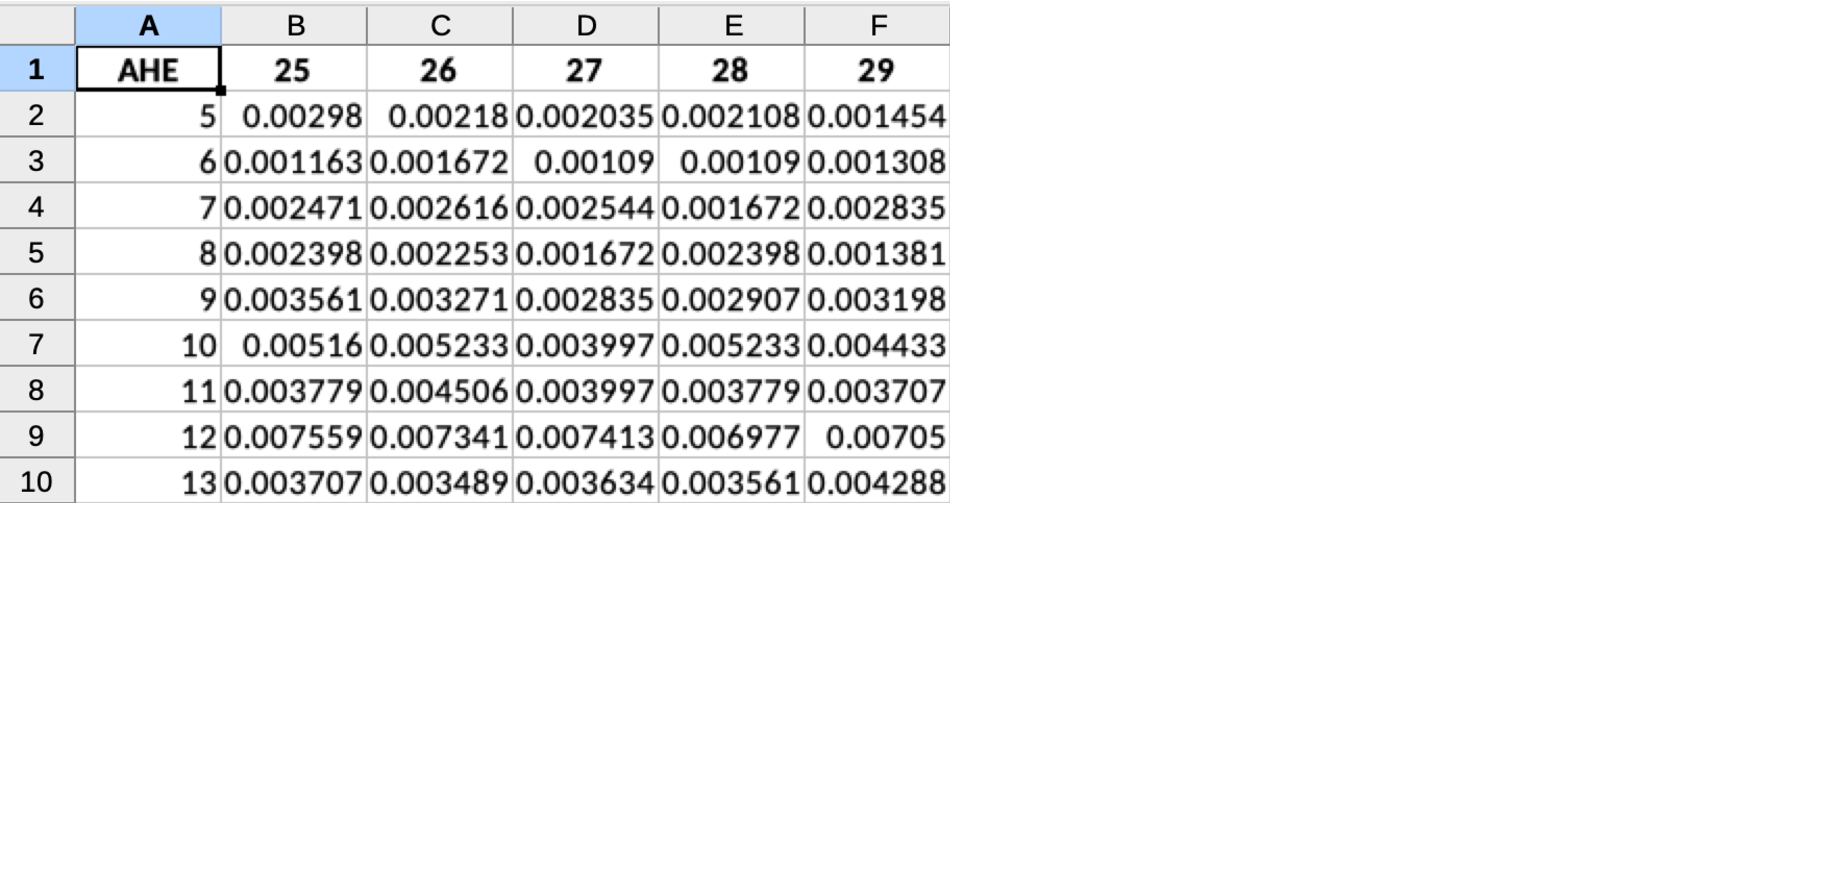
\includegraphics{data-wide-format.pdf}
\end{frame}

\begin{frame}{Long Format}
\protect\hypertarget{long-format}{}
This is what data in long format looks like:

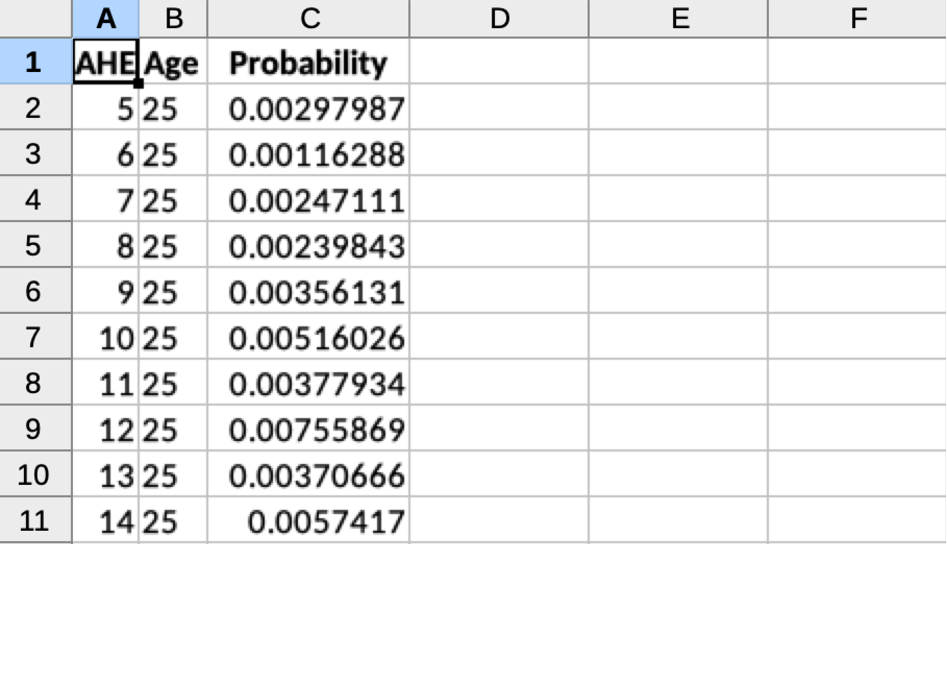
\includegraphics{data-long-format.pdf}
\end{frame}

\begin{frame}{Marginal Distribution}
\protect\hypertarget{marginal-distribution}{}
The general expression for the marginal distribution: \[
\text{Pr}(Y=y) = \sum_{i=1}^n \text{Pr}(X=x_i, Y=y)
\] In particular, for \(Age=25\), we have \[
\text{Pr}(Age=25) = \sum_{ahe=5}^{70} \text{Pr}(AHE=ahe, Age=25)
\] We can now calculate these conveniently with the long-form dataframe.
\end{frame}

\begin{frame}[fragile]{Marginal Distribution}
\protect\hypertarget{marginal-distribution-1}{}
Add up the probabilities by Age, using the long-form dataframe:

\footnotesize

\begin{Shaded}
\begin{Highlighting}[]
\FunctionTok{sum}\NormalTok{(df2[df2}\SpecialCharTok{$}\NormalTok{Age }\SpecialCharTok{==} \DecValTok{25}\NormalTok{,]}\SpecialCharTok{$}\NormalTok{Probability)}
\CommentTok{\#\textgreater{} [1] 0.0849}
\FunctionTok{sum}\NormalTok{(df2[df2}\SpecialCharTok{$}\NormalTok{Age }\SpecialCharTok{==} \DecValTok{26}\NormalTok{,]}\SpecialCharTok{$}\NormalTok{Probability)}
\CommentTok{\#\textgreater{} [1] 0.0922}
\FunctionTok{sum}\NormalTok{(df2[df2}\SpecialCharTok{$}\NormalTok{Age }\SpecialCharTok{==} \DecValTok{27}\NormalTok{,]}\SpecialCharTok{$}\NormalTok{Probability)}
\CommentTok{\#\textgreater{} [1] 0.0855}
\FunctionTok{sum}\NormalTok{(df2[df2}\SpecialCharTok{$}\NormalTok{Age }\SpecialCharTok{==} \DecValTok{28}\NormalTok{,]}\SpecialCharTok{$}\NormalTok{Probability)}
\CommentTok{\#\textgreater{} [1] 0.0934}
\FunctionTok{sum}\NormalTok{(df2[df2}\SpecialCharTok{$}\NormalTok{Age }\SpecialCharTok{==} \DecValTok{29}\NormalTok{,]}\SpecialCharTok{$}\NormalTok{Probability)}
\CommentTok{\#\textgreater{} [1] 0.103}
\FunctionTok{sum}\NormalTok{(df2[df2}\SpecialCharTok{$}\NormalTok{Age }\SpecialCharTok{==} \DecValTok{30}\NormalTok{,]}\SpecialCharTok{$}\NormalTok{Probability)}
\CommentTok{\#\textgreater{} [1] 0.105}
\FunctionTok{sum}\NormalTok{(df2[df2}\SpecialCharTok{$}\NormalTok{Age }\SpecialCharTok{==} \DecValTok{31}\NormalTok{,]}\SpecialCharTok{$}\NormalTok{Probability)}
\CommentTok{\#\textgreater{} [1] 0.104}
\FunctionTok{sum}\NormalTok{(df2[df2}\SpecialCharTok{$}\NormalTok{Age }\SpecialCharTok{==} \DecValTok{32}\NormalTok{,]}\SpecialCharTok{$}\NormalTok{Probability)}
\CommentTok{\#\textgreater{} [1] 0.108}
\FunctionTok{sum}\NormalTok{(df2[df2}\SpecialCharTok{$}\NormalTok{Age }\SpecialCharTok{==} \DecValTok{33}\NormalTok{,]}\SpecialCharTok{$}\NormalTok{Probability)}
\CommentTok{\#\textgreater{} [1] 0.109}
\FunctionTok{sum}\NormalTok{(df2[df2}\SpecialCharTok{$}\NormalTok{Age }\SpecialCharTok{==} \DecValTok{34}\NormalTok{,]}\SpecialCharTok{$}\NormalTok{Probability)}
\CommentTok{\#\textgreater{} [1] 0.115}
\end{Highlighting}
\end{Shaded}

\normalsize
\end{frame}

\begin{frame}[fragile]{Marginal Distribution}
\protect\hypertarget{marginal-distribution-2}{}
To avoid copy-pasting, you can use a split/apply technique:

\footnotesize

\begin{Shaded}
\begin{Highlighting}[]
\FunctionTok{sapply}\NormalTok{(}\FunctionTok{split}\NormalTok{(df2, df2}\SpecialCharTok{$}\NormalTok{Age), }\ControlFlowTok{function}\NormalTok{(x) }\FunctionTok{sum}\NormalTok{(x}\SpecialCharTok{$}\NormalTok{Probability))}
\CommentTok{\#\textgreater{}     25     26     27     28     29     30     31     32     33     34 }
\CommentTok{\#\textgreater{} 0.0849 0.0922 0.0855 0.0934 0.1035 0.1047 0.1039 0.1081 0.1088 0.1150}
\end{Highlighting}
\end{Shaded}

\normalsize

And you can always write a loop:

\footnotesize

\begin{Shaded}
\begin{Highlighting}[]
\ControlFlowTok{for}\NormalTok{ (age }\ControlFlowTok{in} \DecValTok{25}\SpecialCharTok{:}\DecValTok{34}\NormalTok{)\{}
    \FunctionTok{print}\NormalTok{(}\FunctionTok{sum}\NormalTok{(df2[df2}\SpecialCharTok{$}\NormalTok{Age }\SpecialCharTok{==}\NormalTok{ age,]}\SpecialCharTok{$}\NormalTok{Probability))}
\NormalTok{\}}
\CommentTok{\#\textgreater{} [1] 0.0849}
\CommentTok{\#\textgreater{} [1] 0.0922}
\CommentTok{\#\textgreater{} [1] 0.0855}
\CommentTok{\#\textgreater{} [1] 0.0934}
\CommentTok{\#\textgreater{} [1] 0.103}
\CommentTok{\#\textgreater{} [1] 0.105}
\CommentTok{\#\textgreater{} [1] 0.104}
\CommentTok{\#\textgreater{} [1] 0.108}
\CommentTok{\#\textgreater{} [1] 0.109}
\CommentTok{\#\textgreater{} [1] 0.115}
\end{Highlighting}
\end{Shaded}

\normalsize
\end{frame}

\begin{frame}[fragile]{Marginal Distribution}
\protect\hypertarget{marginal-distribution-3}{}
Using data in wide format is sometimes convenient.

Add up for all MHE rows:

\footnotesize

\begin{Shaded}
\begin{Highlighting}[]
\FunctionTok{colSums}\NormalTok{(df1[,}\FunctionTok{names}\NormalTok{(df1) }\SpecialCharTok{!=} \StringTok{"AHE"}\NormalTok{])}
\CommentTok{\#\textgreater{}     25     26     27     28     29     30     31     32     33     34 }
\CommentTok{\#\textgreater{} 0.0849 0.0922 0.0855 0.0934 0.1035 0.1047 0.1039 0.1081 0.1088 0.1150}
\end{Highlighting}
\end{Shaded}

\normalsize

Add up for all Age columns, using the wide-form dataframe:

\footnotesize

\begin{Shaded}
\begin{Highlighting}[]
\FunctionTok{rowSums}\NormalTok{(df1[,}\FunctionTok{names}\NormalTok{(df1) }\SpecialCharTok{!=} \StringTok{"AHE"}\NormalTok{])}
\CommentTok{\#\textgreater{}  [1] 0.01708 0.01192 0.02202 0.02115 0.02784 0.04572 0.03474 0.06985 0.03743}
\CommentTok{\#\textgreater{} [10] 0.06301 0.04041 0.03249 0.05669 0.02842 0.05909 0.03590 0.05233 0.06766}
\CommentTok{\#\textgreater{} [19] 0.03649 0.04150 0.04237 0.04862 0.03125 0.02144 0.01773 0.00858 0.00974}
\CommentTok{\#\textgreater{} [28] 0.00443 0.01410}
\end{Highlighting}
\end{Shaded}

\normalsize

Note that:

\footnotesize

\begin{Shaded}
\begin{Highlighting}[]
\FunctionTok{sum}\NormalTok{(}\FunctionTok{colSums}\NormalTok{(df1[,}\FunctionTok{names}\NormalTok{(df1) }\SpecialCharTok{!=} \StringTok{"AHE"}\NormalTok{]))}
\CommentTok{\#\textgreater{} [1] 1}
\end{Highlighting}
\end{Shaded}

\normalsize
\end{frame}

\begin{frame}[fragile]{Save your results}
\protect\hypertarget{save-your-results}{}
You may want to append your results to the original data, the way you
would in a spreadsheet. This may be convenient if you plan to save the
data in a spreadsheet at the end of the project.

To avoid altering the clean dataframe \texttt{df1}, let's make a copy
first:

\footnotesize

\begin{Shaded}
\begin{Highlighting}[]
\NormalTok{d }\OtherTok{\textless{}{-}}\NormalTok{ df1  }\CommentTok{\# make a copy to preserve original dataframe}
\end{Highlighting}
\end{Shaded}

\normalsize

Append sums to last column:

\footnotesize

\begin{Shaded}
\begin{Highlighting}[]
\NormalTok{d}\SpecialCharTok{$}\NormalTok{Total }\OtherTok{\textless{}{-}} \FunctionTok{rowSums}\NormalTok{(df1[,}\FunctionTok{names}\NormalTok{(df1) }\SpecialCharTok{!=} \StringTok{"AHE"}\NormalTok{])}
\end{Highlighting}
\end{Shaded}

\normalsize

Append sums to last row: add NA to the first column, for alignment

\footnotesize

\begin{Shaded}
\begin{Highlighting}[]
\NormalTok{d }\OtherTok{\textless{}{-}} \FunctionTok{rbind}\NormalTok{(d, }\FunctionTok{c}\NormalTok{(}\ConstantTok{NA}\NormalTok{, }\FunctionTok{colSums}\NormalTok{(d[,}\FunctionTok{names}\NormalTok{(d) }\SpecialCharTok{!=} \StringTok{"AHE"}\NormalTok{])))}
\end{Highlighting}
\end{Shaded}

\normalsize

Save it as a \texttt{csv} file:

\footnotesize

\begin{Shaded}
\begin{Highlighting}[]
\FunctionTok{write.csv}\NormalTok{(d, }\AttributeTok{file=}\StringTok{"Age\_HourlyEarnings\_clean\_wide\_sums.csv"}\NormalTok{)}
\end{Highlighting}
\end{Shaded}

\normalsize

Save it as a \texttt{xlsx} file:

\footnotesize

\begin{Shaded}
\begin{Highlighting}[]
\FunctionTok{library}\NormalTok{(}\StringTok{"writexl"}\NormalTok{)  }\CommentTok{\# remember to install the package first}
\FunctionTok{write\_xlsx}\NormalTok{(d, }\StringTok{"Age\_HourlyEarnings\_clean\_wide\_sums.xlsx"}\NormalTok{)}
\end{Highlighting}
\end{Shaded}

\normalsize

If you haven't set your working directory, run \texttt{getwd()} to see
where the files were saved.
\end{frame}

\begin{frame}[fragile]{Compute Weighted Means by Age: Base R}
\protect\hypertarget{compute-weighted-means-by-age-base-r}{}
Using base R \textbar{} See below for other methods

Here is an approach based on split/apply:

\footnotesize

\begin{Shaded}
\begin{Highlighting}[]
\FunctionTok{sapply}\NormalTok{(}\FunctionTok{split}\NormalTok{(df2, df2}\SpecialCharTok{$}\NormalTok{Age), }\ControlFlowTok{function}\NormalTok{(x) }\FunctionTok{weighted.mean}\NormalTok{(x}\SpecialCharTok{$}\NormalTok{AHE, x}\SpecialCharTok{$}\NormalTok{Probability))}
\CommentTok{\#\textgreater{}   25   26   27   28   29   30   31   32   33   34 }
\CommentTok{\#\textgreater{} 17.6 19.0 19.7 20.2 21.2 21.8 22.6 23.7 23.3 24.1}
\end{Highlighting}
\end{Shaded}

\normalsize

There are many ways to achieve the same result. The \texttt{tidyverse}
offers more intuitive functions for this purpose. We explore them next.
\end{frame}

\begin{frame}[fragile]{Compute Weighted Means by Age: plyr}
\protect\hypertarget{compute-weighted-means-by-age-plyr}{}
The \texttt{dplyr} package is a crowd's favorite:

\footnotesize

\begin{Shaded}
\begin{Highlighting}[]
\FunctionTok{detach}\NormalTok{(}\StringTok{"package:plyr"}\NormalTok{)  }\CommentTok{\# to avoid conflict with dplyr}
\FunctionTok{library}\NormalTok{(}\StringTok{"dplyr"}\NormalTok{)}
\NormalTok{df2 }\SpecialCharTok{\%\textgreater{}\%}
    \FunctionTok{group\_by}\NormalTok{(Age) }\SpecialCharTok{\%\textgreater{}\%}
    \FunctionTok{summarise}\NormalTok{(}\AttributeTok{AHE =} \FunctionTok{weighted.mean}\NormalTok{(AHE, Probability)) }\SpecialCharTok{\%\textgreater{}\%}
    \FunctionTok{head}\NormalTok{(}\DecValTok{5}\NormalTok{)}
\CommentTok{\#\textgreater{} \# A tibble: 5 x 2}
\CommentTok{\#\textgreater{}     Age   AHE}
\CommentTok{\#\textgreater{}   \textless{}int\textgreater{} \textless{}dbl\textgreater{}}
\CommentTok{\#\textgreater{} 1    25  17.6}
\CommentTok{\#\textgreater{} 2    26  19.0}
\CommentTok{\#\textgreater{} 3    27  19.7}
\CommentTok{\#\textgreater{} 4    28  20.2}
\CommentTok{\#\textgreater{} 5    29  21.2}
\end{Highlighting}
\end{Shaded}

\normalsize One advantage of piping is that you can write the variable
name directly --- that is, \texttt{Age} instead of \texttt{df2\$Age}
\end{frame}

\begin{frame}[fragile]{Compute Weighted Means by Age: data.table}
\protect\hypertarget{compute-weighted-means-by-age-data.table}{}
Another popular choice is based on the \texttt{data.table} library. The
\texttt{data.table} library is the most efficient for large datasets.

\footnotesize

\begin{Shaded}
\begin{Highlighting}[]
\FunctionTok{library}\NormalTok{(}\StringTok{"data.table"}\NormalTok{)}
\FunctionTok{head}\NormalTok{(}\FunctionTok{setDT}\NormalTok{(df2)[, .(}\AttributeTok{AHE =} \FunctionTok{weighted.mean}\NormalTok{(AHE, Probability)), Age])}
\CommentTok{\#\textgreater{}    Age  AHE}
\CommentTok{\#\textgreater{} 1:  25 17.6}
\CommentTok{\#\textgreater{} 2:  26 19.0}
\CommentTok{\#\textgreater{} 3:  27 19.7}
\CommentTok{\#\textgreater{} 4:  28 20.2}
\CommentTok{\#\textgreater{} 5:  29 21.2}
\CommentTok{\#\textgreater{} 6:  30 21.8}
\end{Highlighting}
\end{Shaded}

\normalsize
\end{frame}

\begin{frame}{Law of Iterated Expectations}
\protect\hypertarget{law-of-iterated-expectations}{}
In general, \[
E[Y] = \sum_{i=1}^n E[Y|X=x_i]\ \text{Pr}(X=x_i)
\] In particular, \[
E[AHE] = \sum_{age=25}^{34} E[AHE|Age=age]\ \text{Pr}(Age=age)
\]
\end{frame}

\begin{frame}[fragile]{Compute Variance by Age}
\protect\hypertarget{compute-variance-by-age}{}
Similar to what we did with the function \texttt{weighted.mean}, but
here we roll our own \texttt{weighted.variance}:

\footnotesize

\begin{Shaded}
\begin{Highlighting}[]
\NormalTok{weighted.variance }\OtherTok{\textless{}{-}} \ControlFlowTok{function}\NormalTok{(x,w) }\FunctionTok{sum}\NormalTok{(w}\SpecialCharTok{*}\NormalTok{(x}\SpecialCharTok{{-}}\FunctionTok{weighted.mean}\NormalTok{(x,w))}\SpecialCharTok{\^{}}\DecValTok{2}\NormalTok{)}\SpecialCharTok{/}\FunctionTok{sum}\NormalTok{(w)}
\NormalTok{dv }\OtherTok{\textless{}{-}} \FunctionTok{sapply}\NormalTok{(}\FunctionTok{split}\NormalTok{(df2, df2}\SpecialCharTok{$}\NormalTok{Age), }\ControlFlowTok{function}\NormalTok{(x) }\FunctionTok{weighted.variance}\NormalTok{(x}\SpecialCharTok{$}\NormalTok{AHE, x}\SpecialCharTok{$}\NormalTok{Probability))}
\FunctionTok{head}\NormalTok{(dv)}
\CommentTok{\#\textgreater{}    25    26    27    28    29    30 }
\CommentTok{\#\textgreater{}  95.9 129.0 128.8 142.7 152.2 162.8}
\end{Highlighting}
\end{Shaded}

\normalsize As information about the sample size is not available, we do
not attempt to remove any bias that may be present in the formula.
\end{frame}

\begin{frame}[fragile]{Compute Variance for all Ages}
\protect\hypertarget{compute-variance-for-all-ages}{}
To compute the variance for all ages, we first save the mean computed
earlier and merge with the variance computed above.

\footnotesize

\begin{Shaded}
\begin{Highlighting}[]
\NormalTok{df2 }\SpecialCharTok{\%\textgreater{}\%} \FunctionTok{group\_by}\NormalTok{(Age) }\SpecialCharTok{\%\textgreater{}\%}
\NormalTok{    dplyr}\SpecialCharTok{::}\FunctionTok{summarise}\NormalTok{(}\AttributeTok{Probability =} \FunctionTok{sum}\NormalTok{(Probability)) }\OtherTok{{-}\textgreater{}}\NormalTok{ df}

\NormalTok{df2 }\SpecialCharTok{\%\textgreater{}\%} \FunctionTok{group\_by}\NormalTok{(Age) }\SpecialCharTok{\%\textgreater{}\%}
\NormalTok{    dplyr}\SpecialCharTok{::}\FunctionTok{summarise}\NormalTok{(}\AttributeTok{Mean =} \FunctionTok{weighted.mean}\NormalTok{(AHE, Probability)) }\SpecialCharTok{\%\textgreater{}\%}
    \FunctionTok{left\_join}\NormalTok{(df, }\AttributeTok{by =} \StringTok{"Age"}\NormalTok{) }\OtherTok{{-}\textgreater{}}\NormalTok{ df}

\NormalTok{df2 }\SpecialCharTok{\%\textgreater{}\%} \FunctionTok{group\_by}\NormalTok{(Age) }\SpecialCharTok{\%\textgreater{}\%}
\NormalTok{    dplyr}\SpecialCharTok{::}\FunctionTok{summarise}\NormalTok{(}\AttributeTok{Var =} \FunctionTok{weighted.variance}\NormalTok{(AHE, Probability)) }\SpecialCharTok{\%\textgreater{}\%}
    \FunctionTok{left\_join}\NormalTok{(df, }\AttributeTok{by =} \StringTok{"Age"}\NormalTok{) }\OtherTok{{-}\textgreater{}}\NormalTok{ df}

\FunctionTok{head}\NormalTok{(df, }\DecValTok{3}\NormalTok{)}
\CommentTok{\#\textgreater{} \# A tibble: 3 x 4}
\CommentTok{\#\textgreater{}     Age   Var  Mean Probability}
\CommentTok{\#\textgreater{}   \textless{}int\textgreater{} \textless{}dbl\textgreater{} \textless{}dbl\textgreater{}       \textless{}dbl\textgreater{}}
\CommentTok{\#\textgreater{} 1    25  95.9  17.6      0.0849}
\CommentTok{\#\textgreater{} 2    26 129.   19.0      0.0922}
\CommentTok{\#\textgreater{} 3    27 129.   19.7      0.0855}
\end{Highlighting}
\end{Shaded}

\normalsize
\end{frame}

\begin{frame}[fragile]{Compute Variance for all Ages}
\protect\hypertarget{compute-variance-for-all-ages-1}{}
We can now compute the weighted mean and weighted variance:

\footnotesize

\begin{Shaded}
\begin{Highlighting}[]
\NormalTok{df }\SpecialCharTok{\%\textgreater{}\%} \FunctionTok{summarize}\NormalTok{(}\AttributeTok{Mean =} \FunctionTok{weighted.mean}\NormalTok{(Mean, Probability)}\SpecialCharTok{/}\FunctionTok{sum}\NormalTok{(Probability))}
\CommentTok{\#\textgreater{}   Mean}
\CommentTok{\#\textgreater{} 1 21.5}

\NormalTok{df }\SpecialCharTok{\%\textgreater{}\%} \FunctionTok{summarize}\NormalTok{(}\AttributeTok{Var =} \FunctionTok{weighted.mean}\NormalTok{(Var, Probability)}\SpecialCharTok{/}\FunctionTok{sum}\NormalTok{(Probability))}
\CommentTok{\#\textgreater{}   Var}
\CommentTok{\#\textgreater{} 1 161}
\end{Highlighting}
\end{Shaded}

\normalsize

The expected value of the square could be computed likewise

\footnotesize

\begin{Shaded}
\begin{Highlighting}[]
\NormalTok{weighted.squared.exp }\OtherTok{\textless{}{-}} \ControlFlowTok{function}\NormalTok{(x,w) }\FunctionTok{sum}\NormalTok{(w}\SpecialCharTok{*}\NormalTok{x}\SpecialCharTok{\^{}}\DecValTok{2}\NormalTok{)}\SpecialCharTok{/}\FunctionTok{sum}\NormalTok{(w)}
\end{Highlighting}
\end{Shaded}

\normalsize
\end{frame}

\begin{frame}[fragile]{Visualize the Data}
\protect\hypertarget{visualize-the-data}{}
Mean Earnings by Age:

\footnotesize

\begin{Shaded}
\begin{Highlighting}[]
\FunctionTok{library}\NormalTok{(}\StringTok{"ggplot2"}\NormalTok{)}
\FunctionTok{ggplot}\NormalTok{(}\AttributeTok{data=}\NormalTok{dm, }\FunctionTok{aes}\NormalTok{(}\AttributeTok{x=}\NormalTok{Age, }\AttributeTok{y=}\NormalTok{Mean)) }\SpecialCharTok{+}
    \FunctionTok{geom\_point}\NormalTok{() }\SpecialCharTok{+}
    \FunctionTok{ggtitle}\NormalTok{(}\StringTok{"Mean Earnings by Age"}\NormalTok{) }\SpecialCharTok{+}
    \FunctionTok{theme\_bw}\NormalTok{()}
\end{Highlighting}
\end{Shaded}

\normalsize

Variance of Earnings by Age:

\footnotesize

\begin{Shaded}
\begin{Highlighting}[]
\FunctionTok{ggplot}\NormalTok{(}\AttributeTok{data=}\NormalTok{dv, }\FunctionTok{aes}\NormalTok{(}\AttributeTok{x=}\NormalTok{Age, }\AttributeTok{y=}\NormalTok{Variance)) }\SpecialCharTok{+}
    \FunctionTok{geom\_point}\NormalTok{() }\SpecialCharTok{+}
    \FunctionTok{ggtitle}\NormalTok{(}\StringTok{"Variance of Earnings by Age"}\NormalTok{) }\SpecialCharTok{+}
    \FunctionTok{theme\_bw}\NormalTok{()}
\end{Highlighting}
\end{Shaded}

\normalsize
\end{frame}

\begin{frame}{Visualize the Data}
\protect\hypertarget{visualize-the-data-1}{}
\includegraphics{Problems-Statistics-Earnings_files/figure-beamer/scatter-mean-1.pdf}
\end{frame}

\begin{frame}{Visualize the Data}
\protect\hypertarget{visualize-the-data-2}{}
\includegraphics{Problems-Statistics-Earnings_files/figure-beamer/scatter-variance-1.pdf}`
\end{frame}

\end{document}
